\documentclass{article}[a4paper]
\usepackage[a4paper, total={6in, 9.5in}]{geometry}
\usepackage{charter}
\usepackage{xcolor}
\usepackage{graphicx}
\usepackage{float}
\usepackage{listings}
\usepackage{tabularray}
\usepackage{amsmath}
\usepackage{amssymb}
\usepackage{enumitem}
\usepackage[hidelinks]{hyperref}

\lstset{
  language=Python,
  basicstyle=\ttfamily,
  keywordstyle=\color{blue},
  commentstyle=\color{gray},
  stringstyle=\color{red},
  showstringspaces=false,
  columns=fullflexible,
  breaklines=true
}

\title{
	\huge{\textbf{
		Assignment 01
	}}\\
	\Large{
		Learning from Data, Related Challenges, Linear Models for Regression
	}\\
	\large{\phantom{}}\\
	\large{
		submitted for
	}\\
	\LARGE{
		\textbf{EN3150 - Pattern Recognition}
	}\\
	\large{
		Department of Electronic and Telecommunication Engineering
	}
	\\
	\large{University of Moratuwa}
}

\author{
	\textbf{Udugamasooriya P. H. J.}\\
	220658U % \quad - \quad \href{https://github.com/pulasthi-u/en3160-assignment01}{GitHub}\\
}

\date{12 August 2025}

\allowdisplaybreaks

\begin{document}

	\maketitle

	\section{Impact of Outliers on Linear Regression}

	\textbf{Question 02}
	We start by representing the independent variables in a matrix \[
		\mathbf{X} = \begin{pmatrix}
			1		& x_1		\\
			\vdots	& \vdots	\\
			1		& x_n
		\end{pmatrix},
	\] the dependent variables in a vector \[
		\mathbf{y} = \begin{pmatrix}
			y_1 & \cdots & y_n
		\end{pmatrix} ^ \top,
	\] and directly use the result that \[
		\mathbf{w}_\text{OLS}
		=
		\begin{pmatrix} w_0 & w_1 \end{pmatrix} ^ \top
		=
		\underset{\mathbf{w}}{\arg\min}
		\left( \mathbf{y} - \mathbf{X} \mathbf{w} \right)^2
		=
		\left( \mathbf{X}^\top \mathbf{X} \right)^{-1} \mathbf{X}^\top \mathbf{y}.
	\] This yielded the following result:
	\begin{lstlisting}
Ordinary Least Squares Weights (w): [ 3.91672727 -3.55727273]
	\end{lstlisting}
	Hence \[
		\mathbf{w}_\text{OLS} = \begin{pmatrix} 3.91672727 \\ -3.55727273 \end{pmatrix},
	\] and the predicted linear model is \[
		y = 3.91672727 - 3.55727273 x.
	\]
	A plot of the given data points against the predicted values is shown in Figure \ref{q1}.

	\begin{figure}[H]
		\centering
		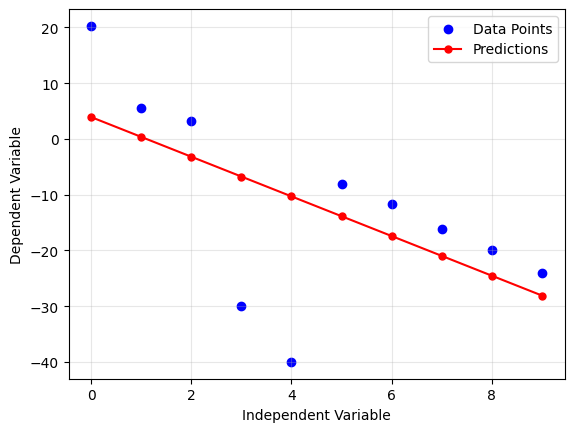
\includegraphics[width=0.7\linewidth]{images/q1.png}
		\caption{abc}
		\label{q1}
	\end{figure}

	\textbf{Question 04} The code in X was used to calculate the loss for each model, for each given value
	of $\beta$. The output of the code was the following:
	\begin{verbatim}
Model 1 : [12 -4]
	 Loss for beta = 1      : 0.435416262490386
	 Loss for beta = 1e-06  : 0.9999999998258207
	 Loss for beta = 1000.0 : 0.0002268287498440988
Model 2 : [ 3.91 -3.55]
	 Loss for beta = 1      : 0.9728470518681676
	 Loss for beta = 1e-06  : 0.9999999999999718
	 Loss for beta = 1000.0 : 0.00018824684654645654
	\end{verbatim}

	Summarizing the results in a table, we have
	\newline

	\begin{tblr}{
		colspec={X[1, c] X[1, c] X[1, c]},
		hlines, vlines
	}
		$\beta$		& Model 1	& Model 2 \\
		$1$			& $0.4354$	& $0.9728$ \\
		$10^{-6}$	& $0.9999$  & $1.0000$ \\
		$10^3$		& $0.0002$  & $0.0002$ \\
	\end{tblr}
	\newline

	\textbf{Question 05} We propose setting $\beta = 1$ to mitigate the impact of outliers.

	\textbf{Question 06} xyz

	\textbf{Question 07} def

	\textbf{Question 08} ghi

	\section{Loss Functions}

	\textbf{Question 01} We calculate the squared error \[
		\text{SE}(\hat{y}_i, y_i) = (\hat{y}_i - y_i)^2
	\] and binary cross entropy \[
		\text{BCE}(\hat{y}_i, y_i) = -y_i \log(\hat{y}_i) - (1 - y_i) \log(1 - \hat{y}_i)
	\] of each predicted value $\hat{y}_i$ against the given corresponding target value $y_i$.
	\newline

	\begin{tblr}{
		colspec={X[1, c] X[1, c] X[1, c] X[1, c]},
		vlines, hlines
	}
		True Value ($y_i$)	& Predicted Value ($\hat{y}_i$)	& $\text{SE}(\hat{y}_i, y_i)$	& $\text{BCE}(\hat{y}_i, y_i)$ \\
		1 					& 0.005 						& 0.9900 						& 5.2983 \\
		1 					& 0.010 						& 0.9801 						& 4.6052 \\
		1 					& 0.050 						& 0.9025 						& 2.9957 \\
		1 					& 0.100 						& 0.8100 						& 2.3026 \\
		1 					& 0.200 						& 0.6400 						& 1.6094 \\
		1 					& 0.300 						& 0.4900 						& 1.2040 \\
		1 					& 0.400 						& 0.3600 						& 0.9163 \\
		1 					& 0.500 						& 0.2500 						& 0.6931 \\
		1 					& 0.600 						& 0.1600 						& 0.5108 \\
		1 					& 0.700 						& 0.0900 						& 0.3567 \\
		1 					& 0.800 						& 0.0400 						& 0.2231 \\
		1 					& 0.900 						& 0.0100 						& 0.1054 \\
		1 					& 1.000 						& 0.0000 						& 0.0000 \\
							& Mean							& 0.4402		 				& 1.4407
	\end{tblr}
	\newline
	
	A plot of the different losses against the predicted values is shown in Figure \ref{q2}.

	\begin{figure}[H]
		\centering
		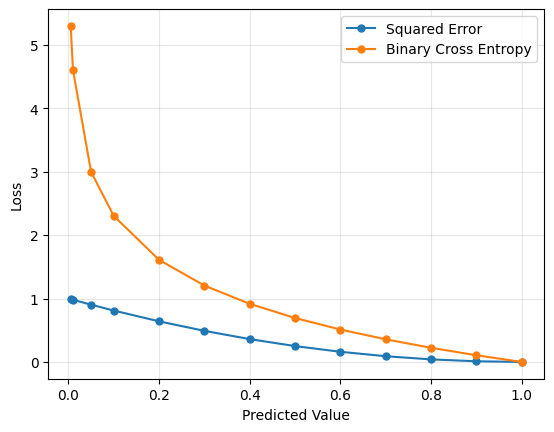
\includegraphics[width=0.7\linewidth]{images/q2.png}
		\caption{abc}
		\label{q2}
	\end{figure}

	\textbf{Question 02}

	\section{Data Pre-Processing}

	\textbf{Question 01} To decide a suitable form of scaling for each feature, we start by visualizing the
	them. The plots in Figure \ref{q3_1} show the distribution of each feature in the dataset.

	\begin{figure}[H]
		\centering
		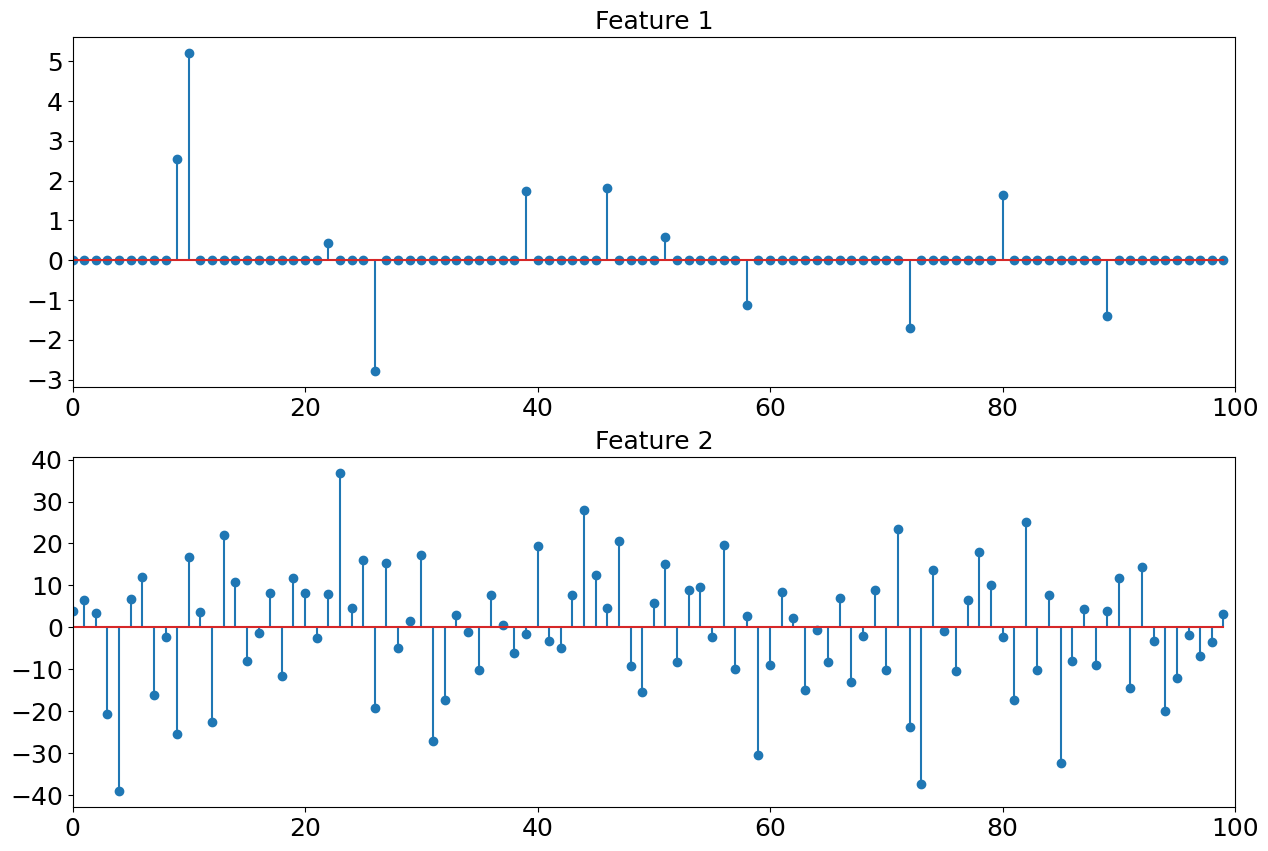
\includegraphics[width=0.7\linewidth]{images/q3_1.png}
		\label{q3_1}
		\caption{abc}
	\end{figure}

	We then run the code in Y to obtain the following summary statistics of each feature:
	\begin{verbatim}
Feature 1
	 Mean 				: 0.06963158220374253
	 Standard Deviation : 0.751690461643816
	 Maximum 			: 5.2
	 Minimum 			: -2.790493210023752
	 Range 				: 7.990493210023752
Feature 2
	 Mean 				: -0.45935709567298505
	 Standard Deviation : 14.351150951654933
	 Maximum 			: 36.752574877667975
	 Minimum 			: -39.11938330852965
	 Range 				: 75.87195818619762
	\end{verbatim}

	Based on the plots above and the above summary statistics, we conclude the following;
	\begin{itemize}
		\item both features have means close to zero
		\item the features vary on different scales, as they have significantly different standard deviations
		\item both features take on both positive and negative values
		\item Feature 1 is sparsely distributed, with most values being equal to 0
	\end{itemize}

	To bring the values of both features to a similar scale, while still preserving the structure and properties of
	each feature, we consider the three following scaling methods;
	\begin{enumerate}
		\item standard scaling,
		\item min-max scaling, and
		\item max-abs scaling.
	\end{enumerate}
	
	We rule out min-max scaling as it would limit both feature values to a range between 0 and 1, affecting the 
	"symmetric" variation among both negative and positive values of both feature values.

	To choose between standard and max-abs scaling, we consider the sparsity of Feature 1. Standard scaling would 
	map the zeros of Feature 1 to non-zero values, resulting in a loss of sparsity, which is a property that
	one would likely want to preserve. Max-abs scaling does not affect sparsity, and maps zeros to zeros. Further, it
	maps to a range between -1 and 1, so negative values map to negative values and positives to positives.

	Hence, we choose max-abs scaling for both feature values. A plot of both feature values after the above scaling
	was applied is shown in Figure \ref{q3_2}. We recalculate the summary statistics for the scaled features too, and
	the results obtained are given below:
	\begin{verbatim}
vab
	\end{verbatim}

\end{document}